\documentclass[11pt]{article}

\usepackage[a4paper, margin=1in]{geometry}
\usepackage{microtype}
\usepackage{amsmath, amssymb, amsthm}
\usepackage{mathtools}
\usepackage{parskip}
\usepackage[hidelinks]{hyperref}
\usepackage{graphicx}
\usepackage{libertinus}

\graphicspath{{figures/}}

\title{Pairing and $k$-NN on a Spiral}
\author{Edvin Tewoldeberhane}
\date{\today}

\begin{document}
\maketitle

Nearest-neighbors regression lets us visualize this transition from a lookup to an average. Fitting a nearest-neighbor algorithm amounts to pairing predictors with outputs. Let's start with the data $X$, drawn from a spiral.

\begin{figure}[h]
    \centering
    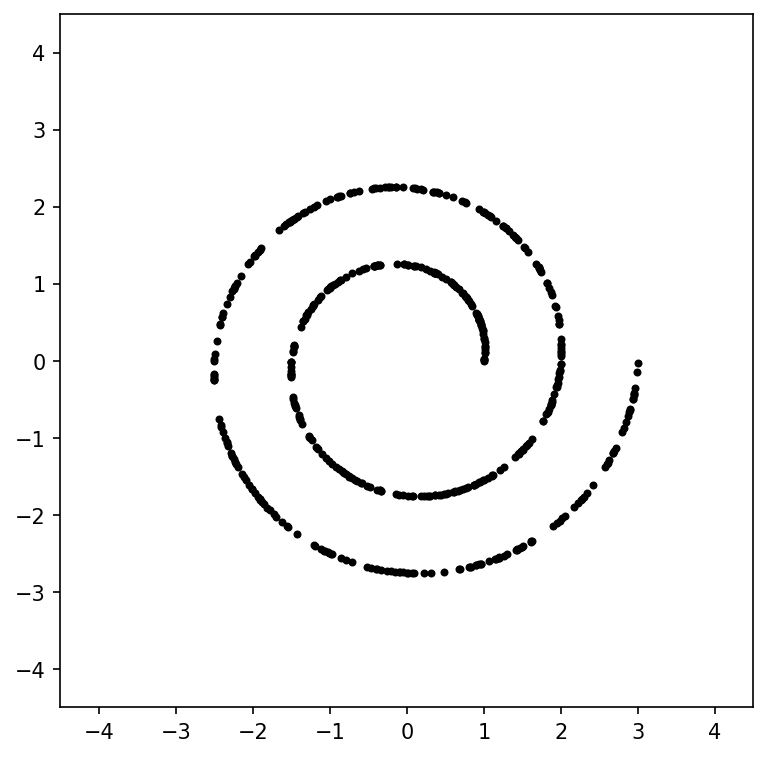
\includegraphics[width=0.55\linewidth]{data.png}
    \caption{Samples $X \sim p_{\text{data}}$ from the spiral.}
\end{figure}

We then sample our own predictors $Z \sim \mathrm{U}(-2, 2)^2$.

\begin{figure}[h]
    \centering
    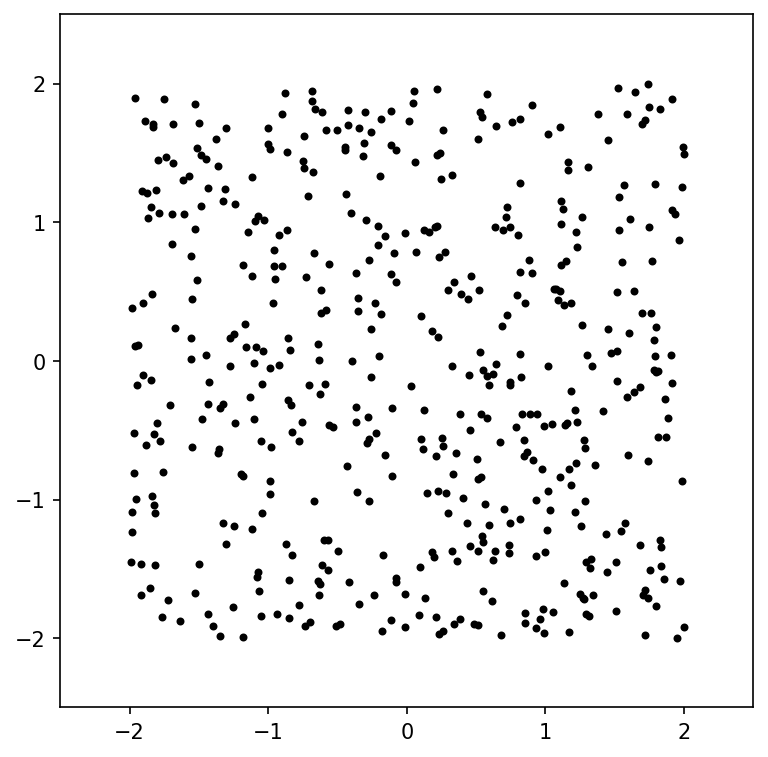
\includegraphics[width=0.55\linewidth]{predictors.png}
    \caption{Predictor samples $Z \sim \mathrm{U}(-2, 2)^2$.}
\end{figure}

Training a $k$-NN regressor amounts to pairing each $z_i$ with an $x_i$. With a
random pairing, the spiral targets are scrambled across the predictor space.

\begin{figure}[h]
    \centering
    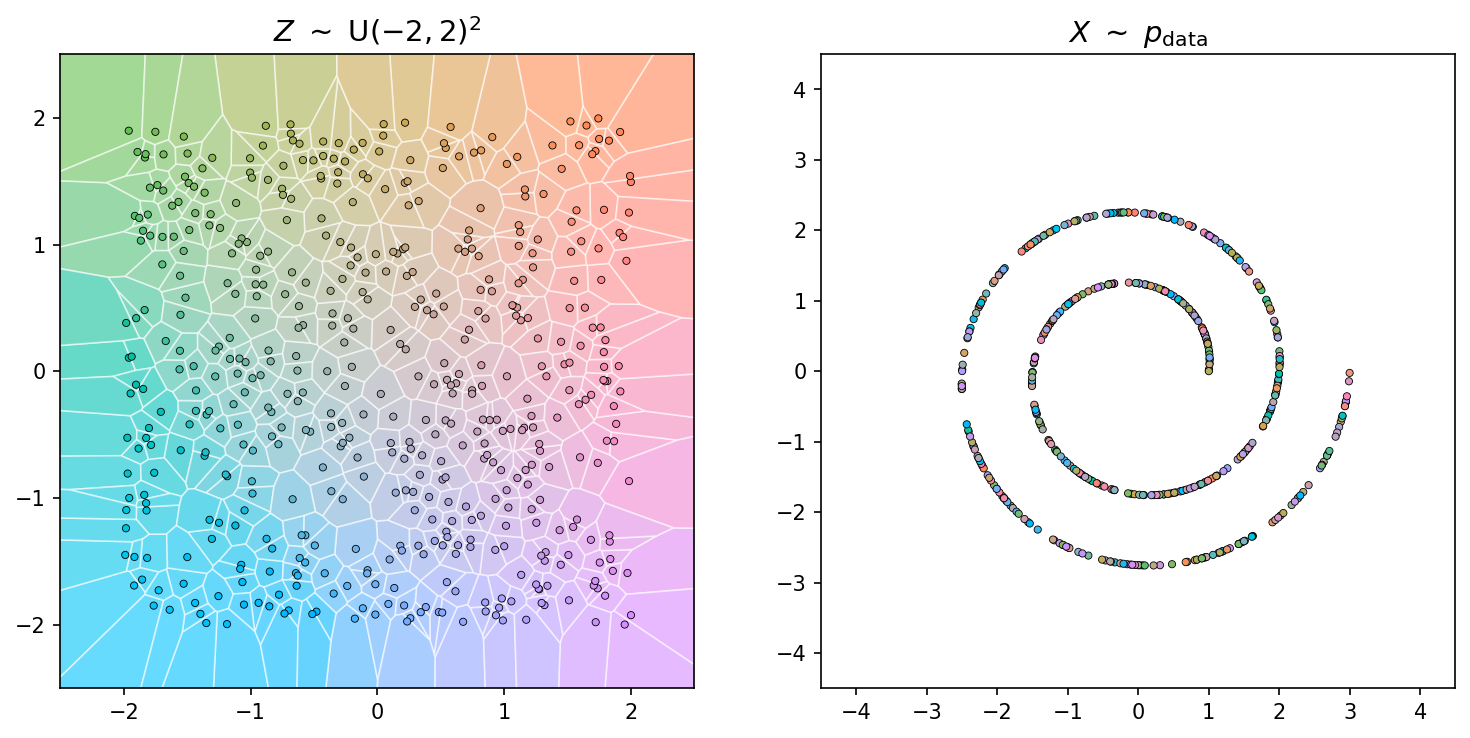
\includegraphics[width=\linewidth]{training.png}
    \caption{Training: each predictor (Voronoi cell on the left) is paired with
    a random data point (right). Matching colors indicate pairing.}
\end{figure}

At inference, a fresh query falls into the Voronoi cell of its nearest training
predictor and inherits the paired target. Averaging more neighbors smooths the
prediction toward the spiral's centroid.

\begin{figure}[h]
    \centering
    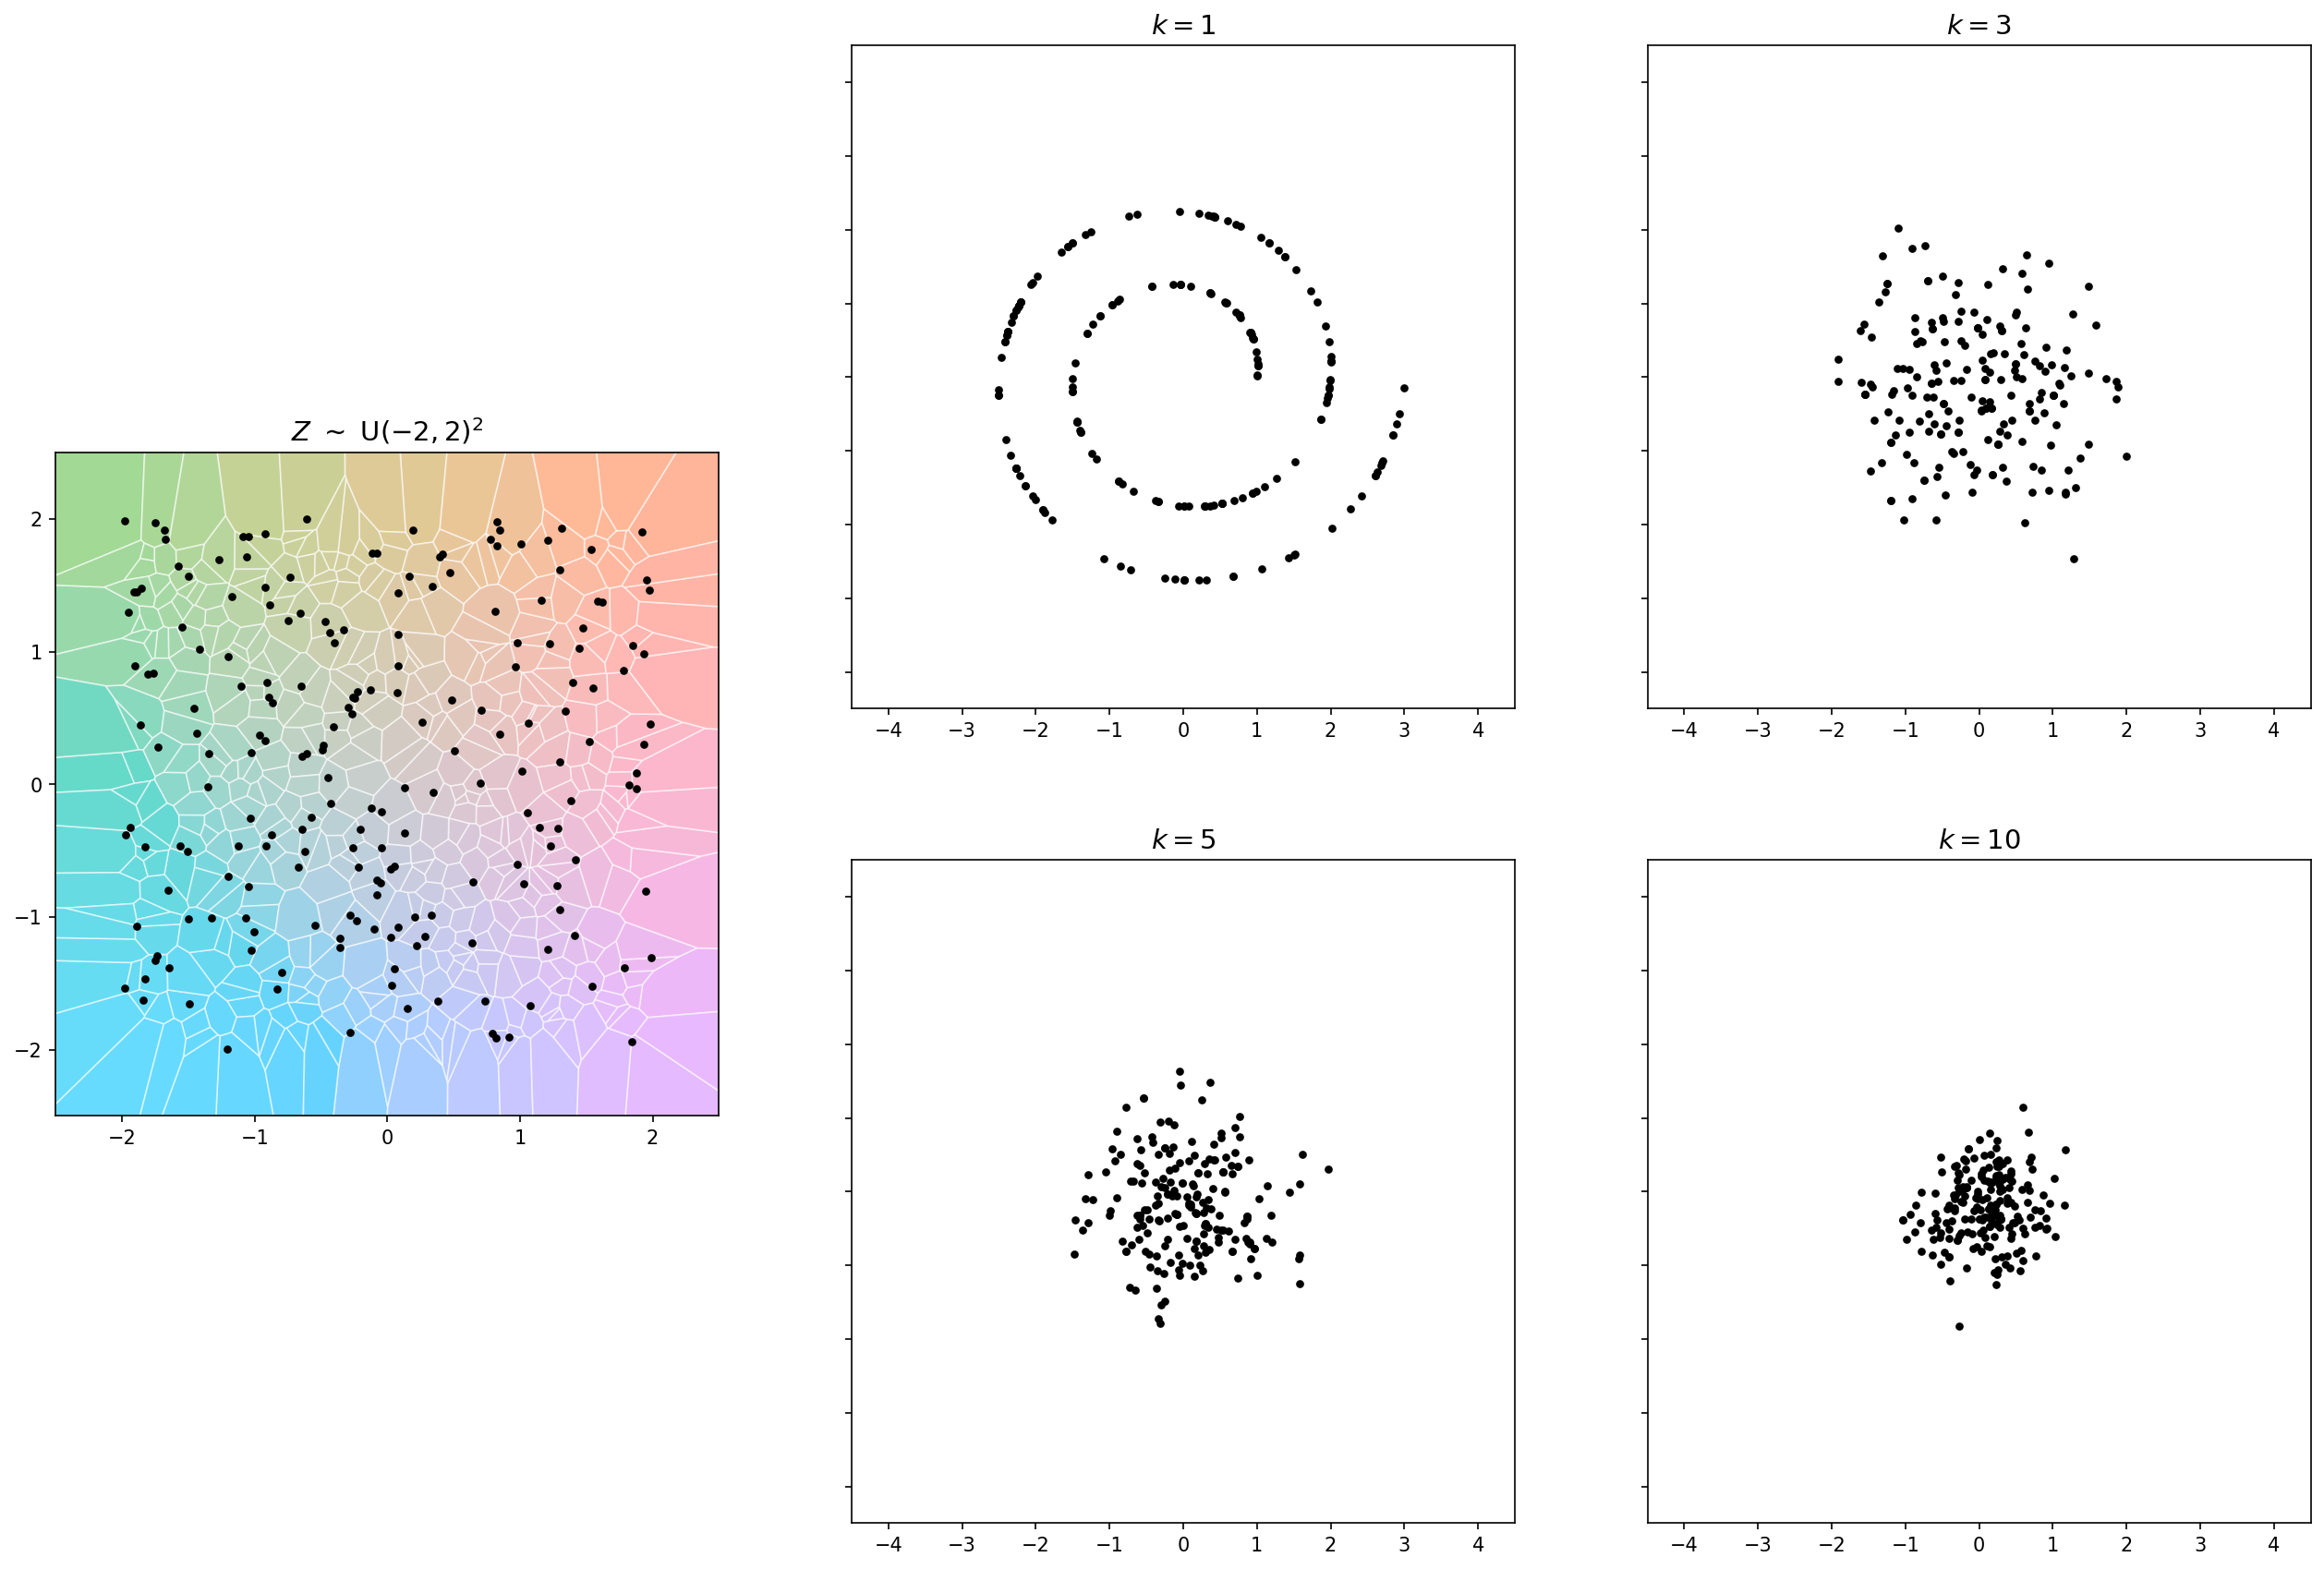
\includegraphics[width=\linewidth]{inference_random.png}
    \caption{Inference under random pairing. New black queries (left) are
    pushed through $k$-NN with $k \in \{1, 3, 5, 10\}$.}
\end{figure}

Re-pairing $z$'s with $x$'s by optimal transport before training produces a
coherent map: nearby predictors get nearby targets. The same $k$-NN now traces
out a recognizable spiral, and even the larger-$k$ averages stay close to the
data manifold.

\begin{figure}[h]
    \centering
    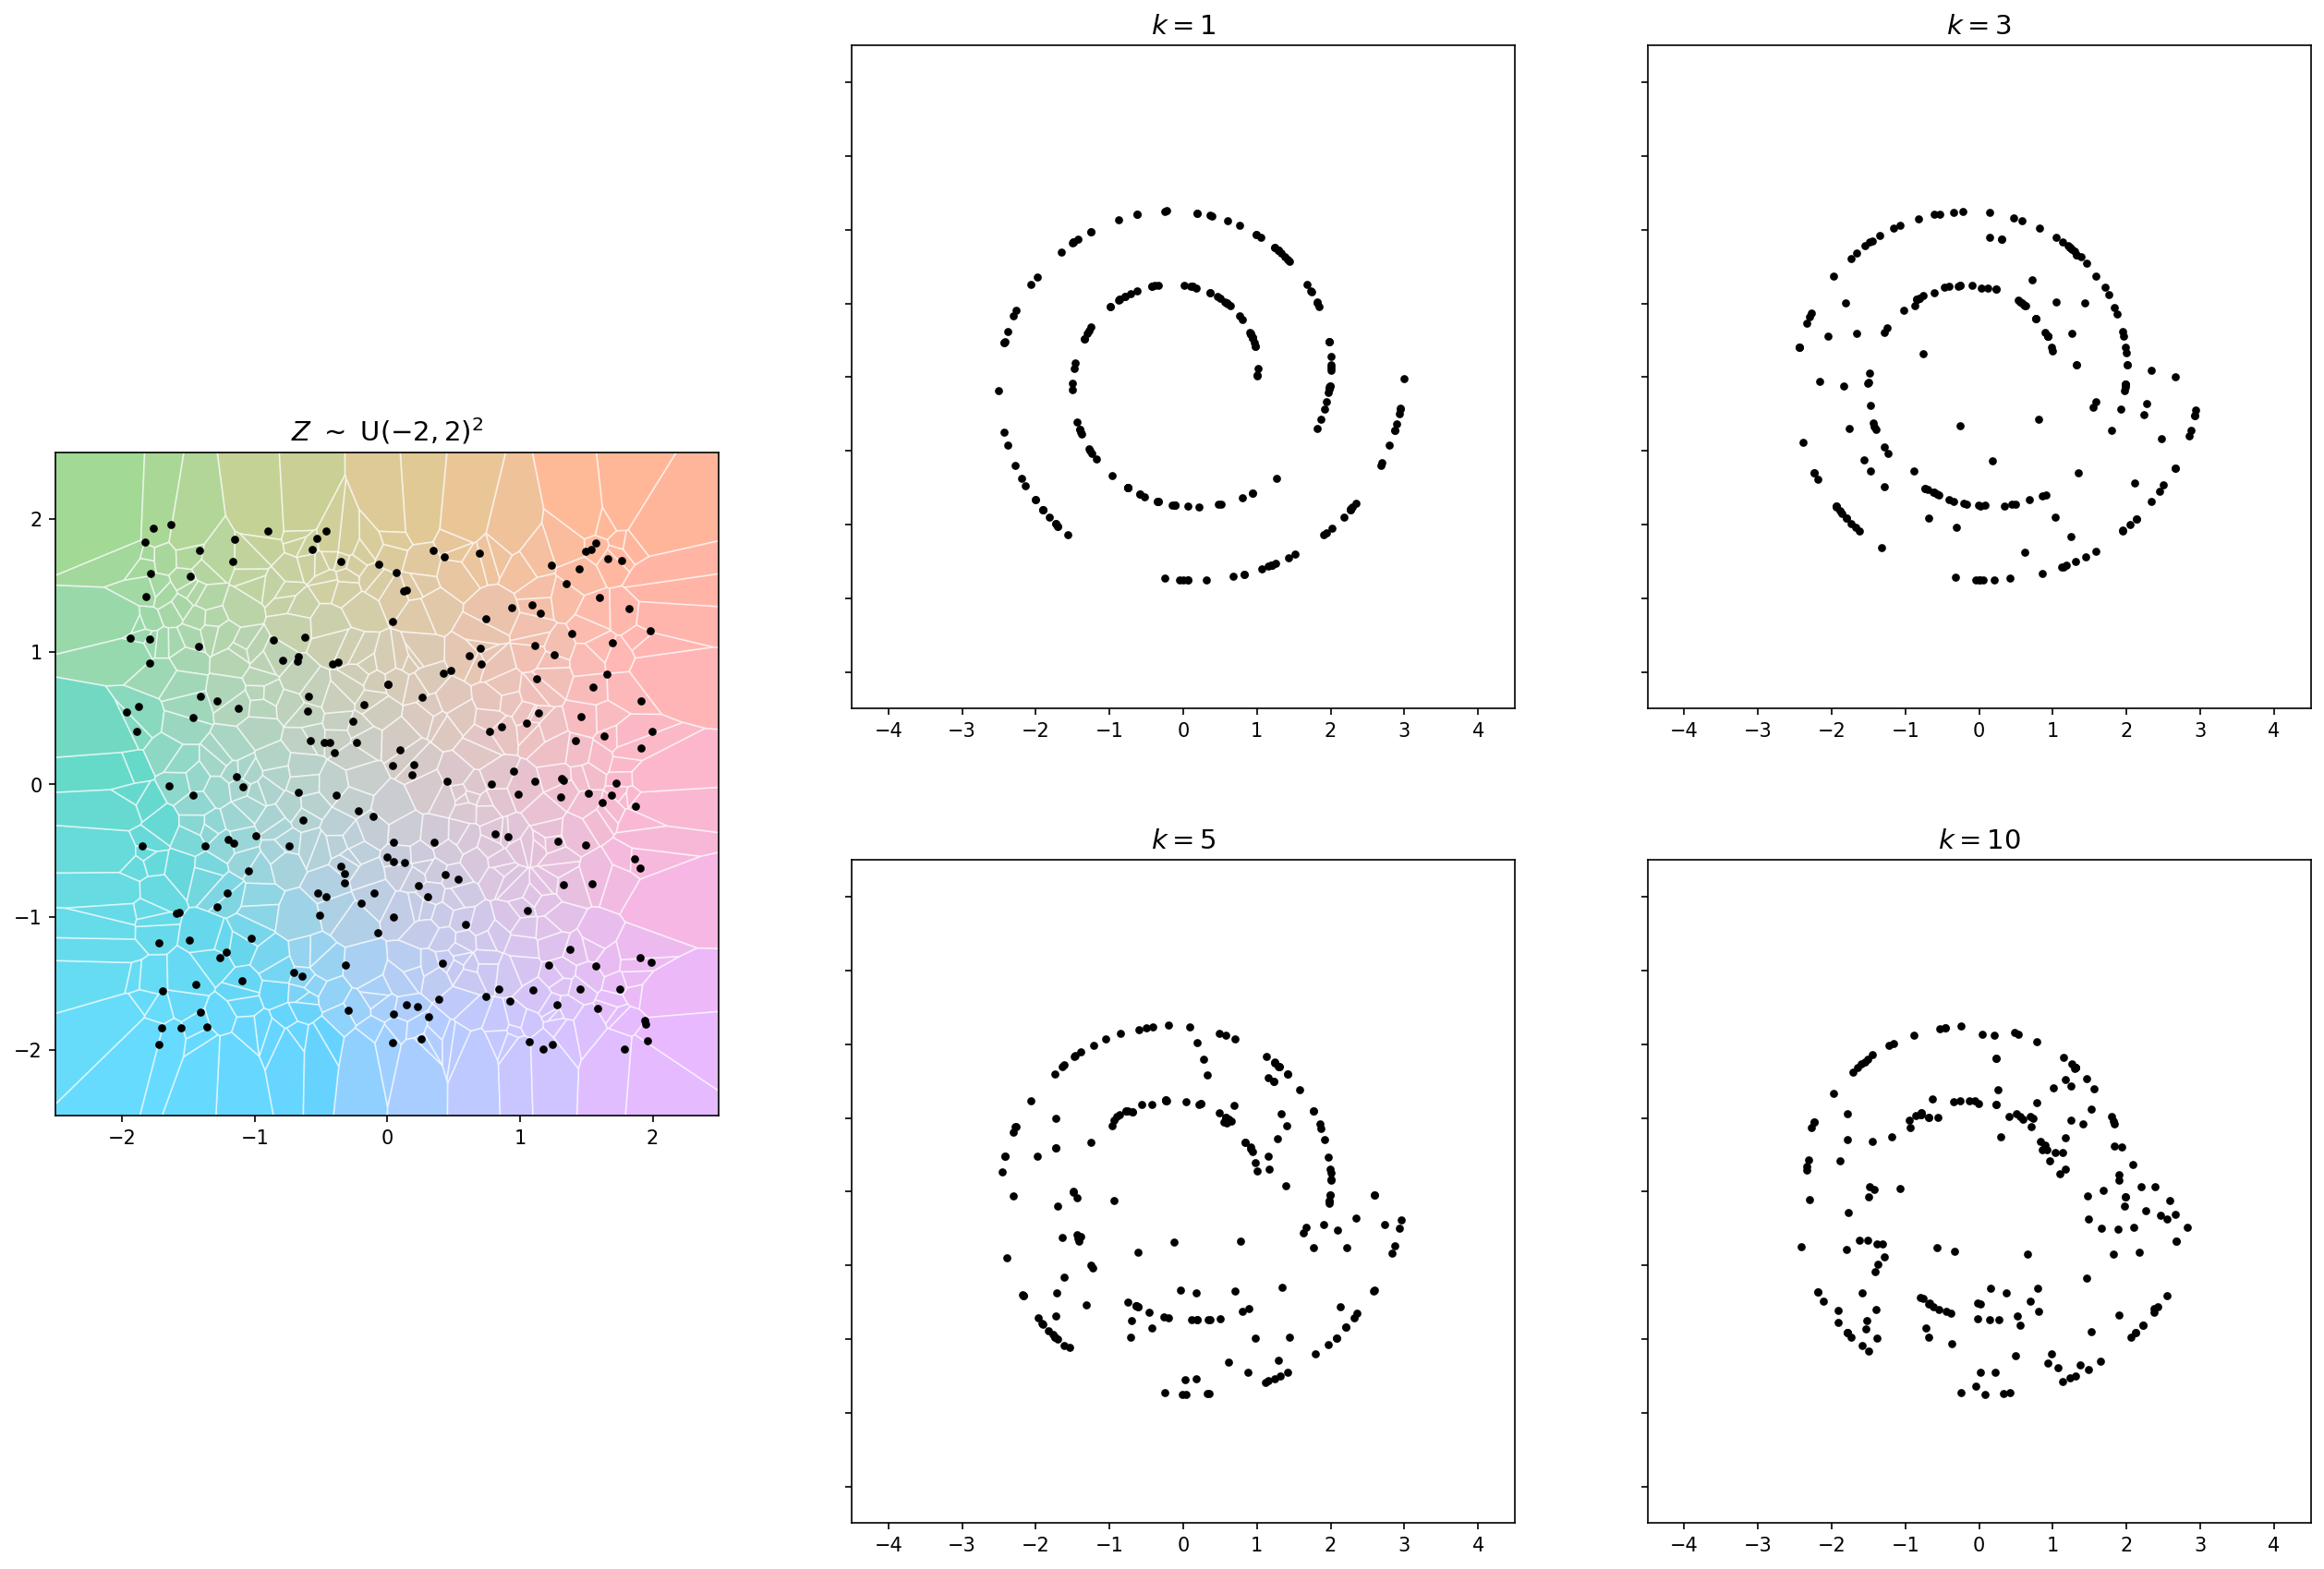
\includegraphics[width=\linewidth]{inference_ot.png}
    \caption{Inference under optimal-transport pairing.}
\end{figure}

\end{document}
